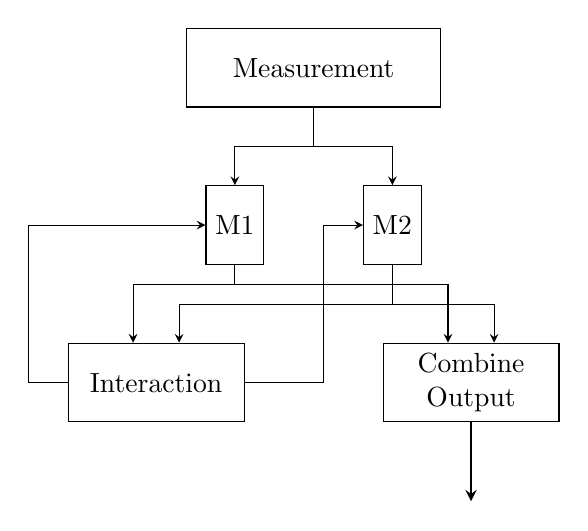
\begin{tikzpicture}[xscale=1,yscale=1,
	square/.style={rectangle, minimum height=10mm, draw=black, align=center},
	round/.style={circle, inner sep=0pt, fill=red!50, opacity=0.75, align=center},
	point/.style={circle, inner sep=0pt, minimum size=2mm, align=center},
	oval/.style={ellipse, fill=gray!50, opacity=0.75},
	label/.style={text width=5mm, align=center},
	node distance= 3cm and 1cm, >=stealth]
	
	%Nodes
	\node[square, text width=30mm]	(measurement)	at (0,0) {Measurement};
	\node[square]	(m1)	at	(-1,-2)	{M1};
	\node[square]	(m2)	at	(1,-2)	{M2};
	\node[square, text width=20mm]	(interact)	at	(-2,-4)	{Interaction};
	\node[square, text width=20mm]	(combine)	at	(2,-4)	{Combine Output};
	
	%Lines
	\draw[black, ->] (measurement.south) -- ++(0,-0.5) -| (m1.north);
	\draw[black, ->] (measurement.south) -- ++(0,-0.5) -| (m2.north);
	\draw[black, ->] (m1.south) -- ++(0,-0.25) -| (interact.120);
	\draw[black, ->] (m1.south) -- ++(0,-0.25) -| (combine.120);
	\draw[black, ->] (m2.south) -- ++(0,-0.5) -| (interact.60);
	\draw[black, ->] (m2.south) -- ++(0,-0.5) -| (combine.60);
	
	\draw[black, ->] (interact.west) -- ++(-0.5,0) |- (m1.west);
	\draw[black, ->] (interact.east) -- ++(1,0) |- (m2.west);
	
	\draw[black, thick, ->] (combine.south) -- ++(0,-1);	
\end{tikzpicture}